% Relative throughput of different coverage feedback mechanisms
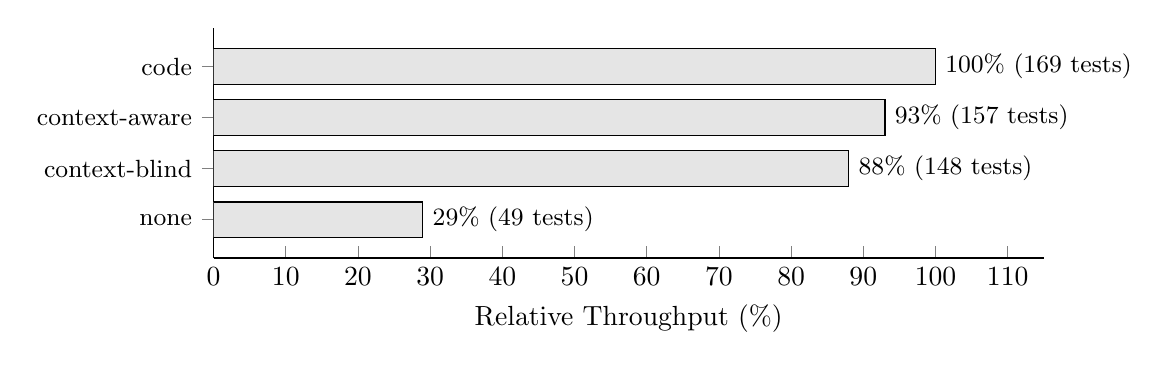
\begin{tikzpicture}
\begin{axis}[
    xbar,
    bar width=0.45cm,
    width=\textwidth,
    height=4.5cm,
    xlabel={Relative Throughput (\%)},
    xmin=0,
    xmax=115,
    ytick=data,
    yticklabels={\propername{code}, \propername{context-aware}, \propername{context-blind}, \propername{none}},
    yticklabel style={font=\small},
    nodes near coords,
    nodes near coords style={font=\small, anchor=west},
    nodes near coords align={horizontal},
    point meta=explicit symbolic,
    axis lines*=left,
    enlarge y limits=0.25,
]
\addplot[fill=gray!20, draw=black, line width=0.4pt] coordinates {
    (100, 3) [100\% (169 tests)]
    (93,  2) [93\% (157 tests)]
    (88,  1) [88\% (148 tests)]
    (29,  0) [29\% (49 tests)]
};
\end{axis}
\end{tikzpicture}